%============================================================
% BAB 2: KAJIAN PUSTAKA
%============================================================
\chapter{KAJIAN PUSTAKA}

Bab ini menguraikan rincian permasalahan pada sistem manajemen rumah kost yang telah dikembangkan sebelumnya, dilanjutkan dengan teori-teori penunjang yang menjadi landasan perancangan ulang arsitektur, serta ulasan penelitian terkait untuk mempertegas posisi dan kebaruan Proyek Akhir ini.

\section{DESKRIPSI PERMASALAHAN}
\label{sec:deskripsi_permasalahan}

Penelitian ini berfokus pada perancangan ulang (\textit{refactoring} / \textit{rewrite}) sistem informasi manajemen rumah kost yang sebelumnya diinisiasi pada Juni 2025 sebagai \textit{previous work} melalui empat proyek akhir terpisah~\cite{rasyidatur2025,roihanah2025,rizal2025,bagus2025}. Pembagian ruang lingkup keempat sistem lama tersebut dirangkum pada Tabel~\ref{tab:sistem_lama}.

\begin{table}[H]
  \centering
  \caption{Penelitian Sistem Lama}
  \label{tab:sistem_lama}
  \begin{tblr}{
    width = \textwidth,
    colspec = {Q[c,0.8cm] X[1.3,l] X[1.2,l] X[2.2,l]}
  }
    No & Proposal / Domain & Peneliti \& NRP & Fokus Awal \\
    1 & Manajemen Penghuni \& Tamu & Rasyidatur (3123500039) & Profil penghuni, buku tamu, dan riwayat sewa~\cite{rasyidatur2025}. \\
    2 & Kamar \& Reservasi & Roihanah (3123500005) & Master kamar, ketersediaan unit, dan validasi bentrok~\cite{roihanah2025}. \\
    3 & Keuangan \& Transaksi & Rizal (3123500060) & Tagihan berkala, pembayaran Midtrans, dan rekap keuangan~\cite{rizal2025}. \\
    4 & Operasional \& Pemeliharaan & Bagus (3123500031) & Tiket komplain kerusakan, inventaris kamar, dan jadwal servis~\cite{bagus2025}. \\
  \end{tblr}
\end{table}

\subsection{Temuan Kelemahan Struktural Sistem Lama}

Meskipun keempat proposal di atas mengusulkan arsitektur modular, penelusuran langsung terhadap kode dan skema basis data sistem lama mengungkap delapan kelemahan struktural yang menjadi dasar perancangan solusi pada Bab~III:

\begin{enumerate}[label=\arabic*., leftmargin=*]
  \item \textbf{Modularitas Semu dan \textit{Tight Coupling} Antar-Domain:}
    Sistem lama membagi domain Penghuni, Kamar, Keuangan, dan Operasional ke dalam folder modul Laravel menggunakan pustaka pihak ketiga, namun pemisahan tersebut tidak ditegakkan oleh kerangka kerja~\cite{alqoran2025}. \textit{Service} pada modul keuangan memanggil langsung model milik modul kamar, dan relasi \textit{Foreign Key} fisik dipasang melintasi batas domain. Akibatnya, perubahan di satu modul berisiko merusak modul lain, dan tidak ada modul yang dapat dipisahkan atau diuji secara mandiri~\cite{alqoran2025}.
  \item \textbf{Model Bisnis Bercabang dan Pembengkakan Basis Data (34 Tabel Domain):}
    Skema basis data sistem lama mencoba melayani varian sewa harian, mingguan, bulanan, dan tahunan sekaligus, lengkap dengan skema uang muka (\textit{down payment}) dan pengembalian dana (\textit{refund}). Model tersebut membuat skema domain membengkak hingga \textbf{34 tabel domain dan RBAC} (serta lebih dari 42 tabel secara keseluruhan di basis data aktual termasuk tabel infrastruktur bawaan \textit{framework}) dengan banyak duplikasi struktur (dua mekanisme penerbitan tagihan antara \texttt{invoices} dan \texttt{guest\_bills}, dua tabel \textit{cache} penghuni aktif antara \texttt{finance\_active\_tenants} dan \texttt{guest\_active\_contexts}, serta tabel gemuk \texttt{room\_schedules} yang mencampur biodata penghuni dengan jadwal sewa)~\cite{roihanah2025,rizal2025}. Pelacakan riwayat transaksi dan pemeliharaan skema pun menjadi rumit~\cite{rizal2025,bagus2025}.
  \item \textbf{Ketiadaan Dukungan Multi-Gedung (\textit{Multi-Tenancy}):}
    Kode dan skema basis data dirancang hanya untuk satu gedung fisik. Ketika pemilik menambah cabang properti baru, tidak ada mekanisme pemisahan data penyewa (\textit{tenant isolation}), sehingga pengembang terpaksa memasang instalasi server dan basis data terpisah untuk tiap gedung. Biaya pemeliharaan ikut berlipat dan laporan keuangan gabungan seluruh properti sulit disusun~\cite{microsoft2025}.
  \item \textbf{Kontrak Respons API Tidak Baku dan Hak Akses Belum Dinamis:}
    Setiap \textit{endpoint} REST mengembalikan struktur JSON yang berbeda-beda pada format \texttt{status}, paginasi, dan pesan kesalahan validasi HTTP 422, sehingga sisi antarmuka web harus menangani setiap kasus secara terpisah~\cite{microsoft2025}. Di sisi otorisasi, hak akses pengguna masih ditanam kaku di dalam kode (\textit{hardcoded}) dan belum dibatasi per gedung, sehingga pengelola satu gedung dapat melihat atau mengubah data gedung lain dan pemilik tidak leluasa mengatur izin staf sesuai tugas lapangan~\cite{rasyidatur2025,roihanah2025,martin2017}.
  \item \textbf{Mekanisme Autentikasi Masih Primitif:}
    Pengelolaan akun hanya memakai autentikasi dasar berupa kombinasi email dan kata sandi. Belum tersedia validasi email saat pendaftaran, pemulihan lupa kata sandi (\textit{forgot password}), pengaturan masa berlaku sesi terstandarisasi, maupun autentikasi dua faktor (\textit{multi-factor authentication}). Selain berisiko terhadap kebocoran akun, waktu pengembangan juga habis terserap untuk membangun fitur autentikasi standar dari nol~\cite{rasyidatur2025,roihanah2025,sakimura2014}.
  \item \textbf{Struktur Antarmuka (\textit{Frontend}) Tidak Terisolasi:}
    Lapisan presentasi (BLoC) pada aplikasi Flutter lama mengakses \textit{repository} secara langsung tanpa perantara \textit{UseCase}. Logika bisnis bercampur dengan komponen antarmuka, sehingga sulit diuji melalui \textit{unit test}~\cite{martin2017}.
  \item \textbf{Integrasi Pembayaran Belum Memenuhi Standar Produksi:}
    Pembayaran digital via Midtrans baru berjalan di lingkungan uji coba (\textit{sandbox}) tanpa pencegahan transaksi ganda (\textit{idempotency key}) dan tanpa verifikasi tanda tangan kriptografis pada \textit{webhook}~\cite{midtrans2025}.
  \item \textbf{Ketiadaan Antarmuka Kueri Cepat Berbasis AI:}
    Untuk mengetahui tingkat keterisian kamar atau total tunggakan sewa, pemilik dan pengelola harus membuka beberapa menu satu per satu secara manual. Sistem lama belum menyediakan antarmuka kueri berbasis \textit{Model Context Protocol} (MCP) yang menghubungkan model kecerdasan buatan (\textit{Large Language Model} / LLM) dengan data operasional secara aman~\cite{anthropic2024}.
\end{enumerate}

\subsection{Evolusi Desain Sistem Sebelum \textit{Rewrite}}
\label{subsec:evolusi_desain}

Bagian ini menyajikan dua artefak desain sistem sebelum \textit{rewrite} (\textit{before}) agar pembaca melihat konteks di balik keputusan arsitektur baru (\textit{after}) yang dirancang pada Subbab~\ref{sec:desain_sistem} dan Subbab~\ref{sec:basis_data} di Bab~III.

\subsubsection{1. Arsitektur Sebelum \textit{Rewrite} (Sistem Lama)}

Sistem lama merupakan gabungan dari \textbf{4 proyek akhir terpisah} yang diimplementasikan menggunakan Laravel dan basis data MySQL dengan pembagian \textbf{8 kelompok modul} (\texttt{Auth/RBAC}, \texttt{Room}, \texttt{Schedule}, \texttt{Finance}, \texttt{Guest}, \texttt{Maintenance}, \texttt{Setting}, dan \texttt{Inventory/Notification}), namun pemisahannya hanya sebatas struktur folder dan tidak ditegakkan kerangka kerja. Modul keuangan masih bisa memanggil langsung model milik modul kamar, dan relasi \textit{Foreign Key} fisik dipasang melintasi batas domain. Seluruh komponen berjalan dalam satu aplikasi monolitik tanpa batas isolasi teknis dan satu basis data MySQL, seperti ditunjukkan pada Gambar~\ref{fig:arsitektur_lama}. Hasil perombakannya menjadi \textbf{1 arsitektur \textit{Modular Monolith} berbasis NestJS berisi 10 modul terenkapsulasi (4 modul \textit{core} dan 6 modul \textit{opsional}, termasuk Modul \texttt{AI / MCP Assistant})} disajikan pada Subbab~\ref{sec:desain_sistem} (Gambar~\ref{fig:arsitektur_terpadu} dan Gambar~\ref{fig:arsitektur_backend}) di Bab~III.

\begin{figure}[H]
  \centering
  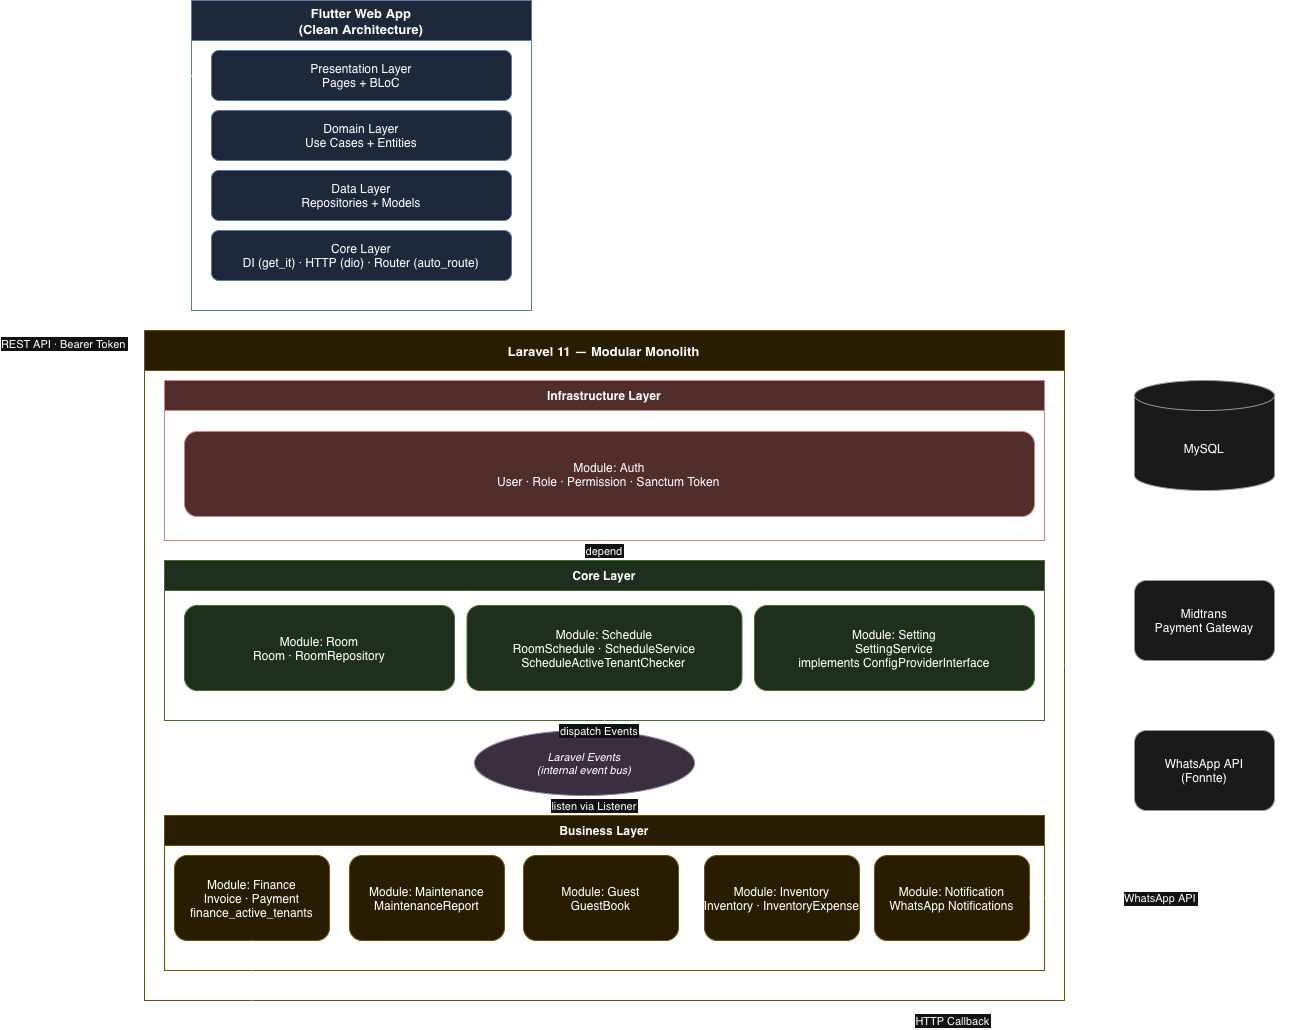
\includegraphics[width=0.95\textwidth,height=0.72\textheight,keepaspectratio]{assets/diagrams/bab2_01_arsitektur_lama.png}
  \caption{Arsitektur Keseluruhan Sistem Sebelum \textit{Rewrite}}
  \label{fig:arsitektur_lama}
\end{figure}

\subsubsection{2. Basis Data Sebelum \textit{Rewrite} (ERD Sistem Lama)}

Karena dirancang untuk mendukung sewa harian, mingguan, bulanan, dan tahunan sekaligus beserta cabang skema \textit{down payment} dan \textit{refund}, basis data domain sistem lama membengkak hingga \textbf{34 tabel domain dan RBAC} dengan berbagai duplikasi tabel turunan serta relasi \textit{Foreign Key} fisik lintas modul. Struktur ERD sistem lama ditunjukkan pada Gambar~\ref{fig:erd_lama}. Penyederhanaan skema 34 tabel ini menjadi rancangan basis data baru yang ramping (\textbf{21 tabel domain utama}), bebas duplikasi, dan tanpa \textit{Foreign Key} lintas modul dibahas rinci pada Subbab~\ref{subsec:erd} (Gambar~\ref{fig:erd_baru}) di Bab~III.

\begin{figure}[H]
  \centering
  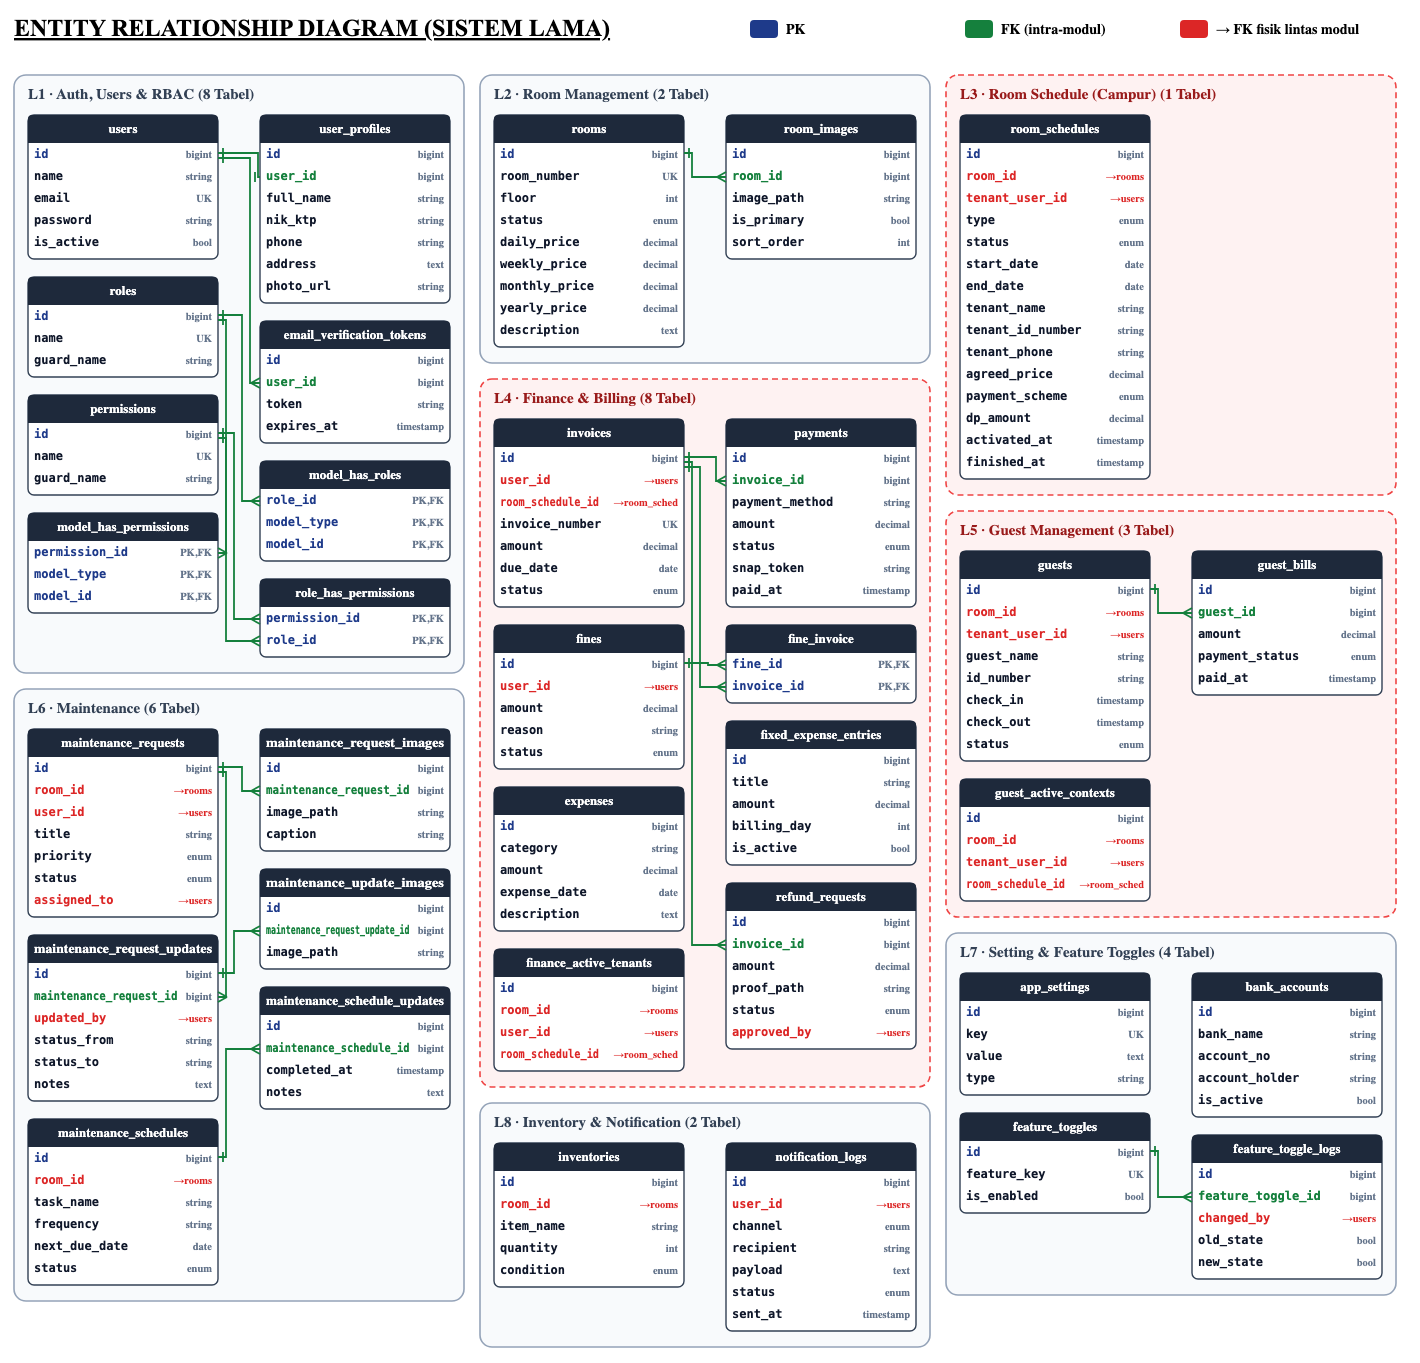
\includegraphics[width=0.98\textwidth,height=0.75\textheight,keepaspectratio]{assets/diagrams/bab2_02_erd_lama.png}
  \caption{Entity Relationship Diagram Sistem Sebelum \textit{Rewrite}}
  \label{fig:erd_lama}
\end{figure}

Perbedaan struktural antara sistem lama (\textit{existing system}) dan sistem baru yang diusulkan dirangkum pada Tabel~\ref{tab:perbandingan_lama_baru}.

\begin{table}[H]
  \centering
  \caption{Perbandingan Sistem Lama (\textit{Existing System}) dan Sistem Baru}
  \label{tab:perbandingan_lama_baru}
  \begin{tblr}{
    width = \textwidth,
    colspec = {X[1.1,l] X[1.8,l] X[1.8,l]}
  }
    Aspek Perbandingan & Sistem Lama (\textit{Existing System}) & Sistem Baru (Usulan Proyek Akhir) \\
    Jumlah \& Struktur Modul & \textbf{4 proyek akhir terpisah} (implementasi gabungan \textbf{8 kelompok modul} hanya sebatas folder tanpa isolasi teknis) & \textbf{1 backend \textit{Modular Monolithic} NestJS} berisi \textbf{10 modul terenkapsulasi} (\textbf{4 \textit{Core} + 6 \textit{Opsional}}) \\
    Komunikasi Antar-Modul & Pemanggilan langsung model lintas modul \& \textit{Foreign Key} fisik lintas domain & Terisolasi via \textbf{\textit{Module Gateway}} dan \textbf{\textit{Event Bus}} tanpa \textit{Foreign Key} fisik lintas modul \\
    Skema Basis Data & \textbf{34 tabel domain \& RBAC} (42+ tabel aktual termasuk tabel infrastruktur), terdapat tabel gemuk \& duplikasi \textit{cache} aktif & \textbf{21 tabel domain utama}, ramping, terisolasi per modul, dan bebas duplikasi \\
    Dukungan Multi-Gedung & \textit{Single-tenant} (1 gedung per instalasi server/basis data) & \textbf{\textit{Multi-Tenant Row-Level Scoping}} (\texttt{building\_id}) dalam 1 basis data terpadu \\
    Autentikasi \& Otorisasi & Email dan kata sandi dasar tanpa verifikasi email/SSO & \textbf{\textit{Single Sign-On} (SSO) Keycloak OIDC}, verifikasi \textit{stateless} JWKS, dan RBAC dinamis \\
    Integrasi Pembayaran & Midtrans \textit{sandbox} tanpa \textit{idempotency key} \& verifikasi \textit{webhook} & Midtrans SNAP siap produksi dengan \textit{idempotency key} dan verifikasi \textit{signature webhook} \\
    Dukungan Asisten AI & Belum tersedia & \textbf{1 Modul Mandiri \texttt{AI / MCP Assistant}} berbasis \textit{Model Context Protocol} (\textit{read-only}) \\
  \end{tblr}
\end{table}

\section{TEORI PENUNJANG}

\subsection{Sistem Informasi Manajemen}

Sistem Informasi Manajemen (SIM) adalah sistem berbasis komputer yang mengumpulkan, menyimpan, mengolah, dan menyajikan data agar dapat dipakai sebagai dasar pengambilan keputusan dalam sebuah organisasi~\cite{tjahjanto2025}. Secara sederhana, SIM mengubah data mentah menjadi informasi yang berguna, lalu informasi itu dipakai untuk perencanaan, pengendalian, dan evaluasi kinerja.

Pada industri properti sewa, SIM menjalankan tiga fungsi yang saling terkait. Pertama, mencatat kondisi fisik properti seperti unit kamar, fasilitas, dan barang di dalamnya. Kedua, merekam seluruh transaksi sewa dari awal kontrak sampai pembayaran terakhir. Ketiga, menyusun laporan keuangan yang bisa dipercaya pemilik sebagai dasar mengambil keputusan.

Proyek Akhir ini memakai konsep SIM sebagai kerangka dasar karena ketiga fungsi tersebut tercakup di dalam sistem yang dibangun. Perbedaan sistem ini dari sistem lama terletak pada otomasi: jika pada sistem lama laporan okupansi dan tunggakan harus dihimpun manual dengan membuka menu satu per satu, pada sistem yang dirancang data langsung tersusun saat masuk sehingga laporan terbentuk otomatis.

\subsection{Arsitektur Modular Monolithic}

Arsitektur modular monolithic membangun aplikasi sebagai satu kesatuan utuh, tetapi membaginya ke dalam modul-modul yang masing-masing punya tanggung jawab dan tidak saling bergantung langsung~\cite{alqoran2025}. Bedanya dengan monolitik konvensional terletak pada pemisahan antar modul. Pada monolitik biasa, pemisahan hanya berupa struktur folder, sehingga \textit{service} di satu bagian tetap bisa memanggil bagian lain tanpa batasan. Pada modular monolithic, pemisahan antar modul ditegakkan dan komunikasi antar modul harus lewat kontrak yang disepakati.

Prinsip batas tersebut diambil dari konsep \textit{bounded context} dalam Domain-Driven Design, yang dipakai untuk menentukan di mana sebuah modul harus berakhir~\cite{dragoni2017}. Setiap modul diperlakukan sebagai satu bagian bisnis dengan aturan main sendiri. Modul keuangan misalnya punya aturan penghitungannya sendiri, dan modul kamar punya aturan tentang ketersediaan unit. Keduanya tidak boleh saling membaca data secara langsung, melainkan berkomunikasi lewat kontrak yang telah ditentukan.

Proyek Akhir ini memakai pendekatan ini karena alasan utamanya adalah kemudahan pemeliharaan ke depan. Ketika bisnis berkembang dan muncul kebutuhan baru, misalnya perlu menambah modul laporan keuangan atau pengarsipan dokumen, penambahan cukup dilakukan dengan membuat modul terpisah dan mendaftarkannya tanpa mengubah modul yang sudah berjalan. Sebaliknya, modul yang tidak lagi dibutuhkan bisa dihapus beserta seluruh isinya tanpa meninggalkan jejak di modul lain.

Kemudahan inilah yang tidak dimiliki sistem lama. Folder modulnya memang ada, tetapi karena batasnya tidak ditegakkan, modul keuangan tetap bisa membaca tabel modul kamar. Akibatnya tidak ada satu pun bagian yang bisa dilepas atau diuji sendiri tanpa melibatkan modul lain. Batas yang benar-benar dipaksakan oleh kerangka kerja membuat penambahan dan penghapusan modul menjadi pekerjaan yang biasa, sebagaimana ditunjukkan pada Gambar~\ref{fig:teori_modulith}.

\begin{figure}[H]
  \centering
  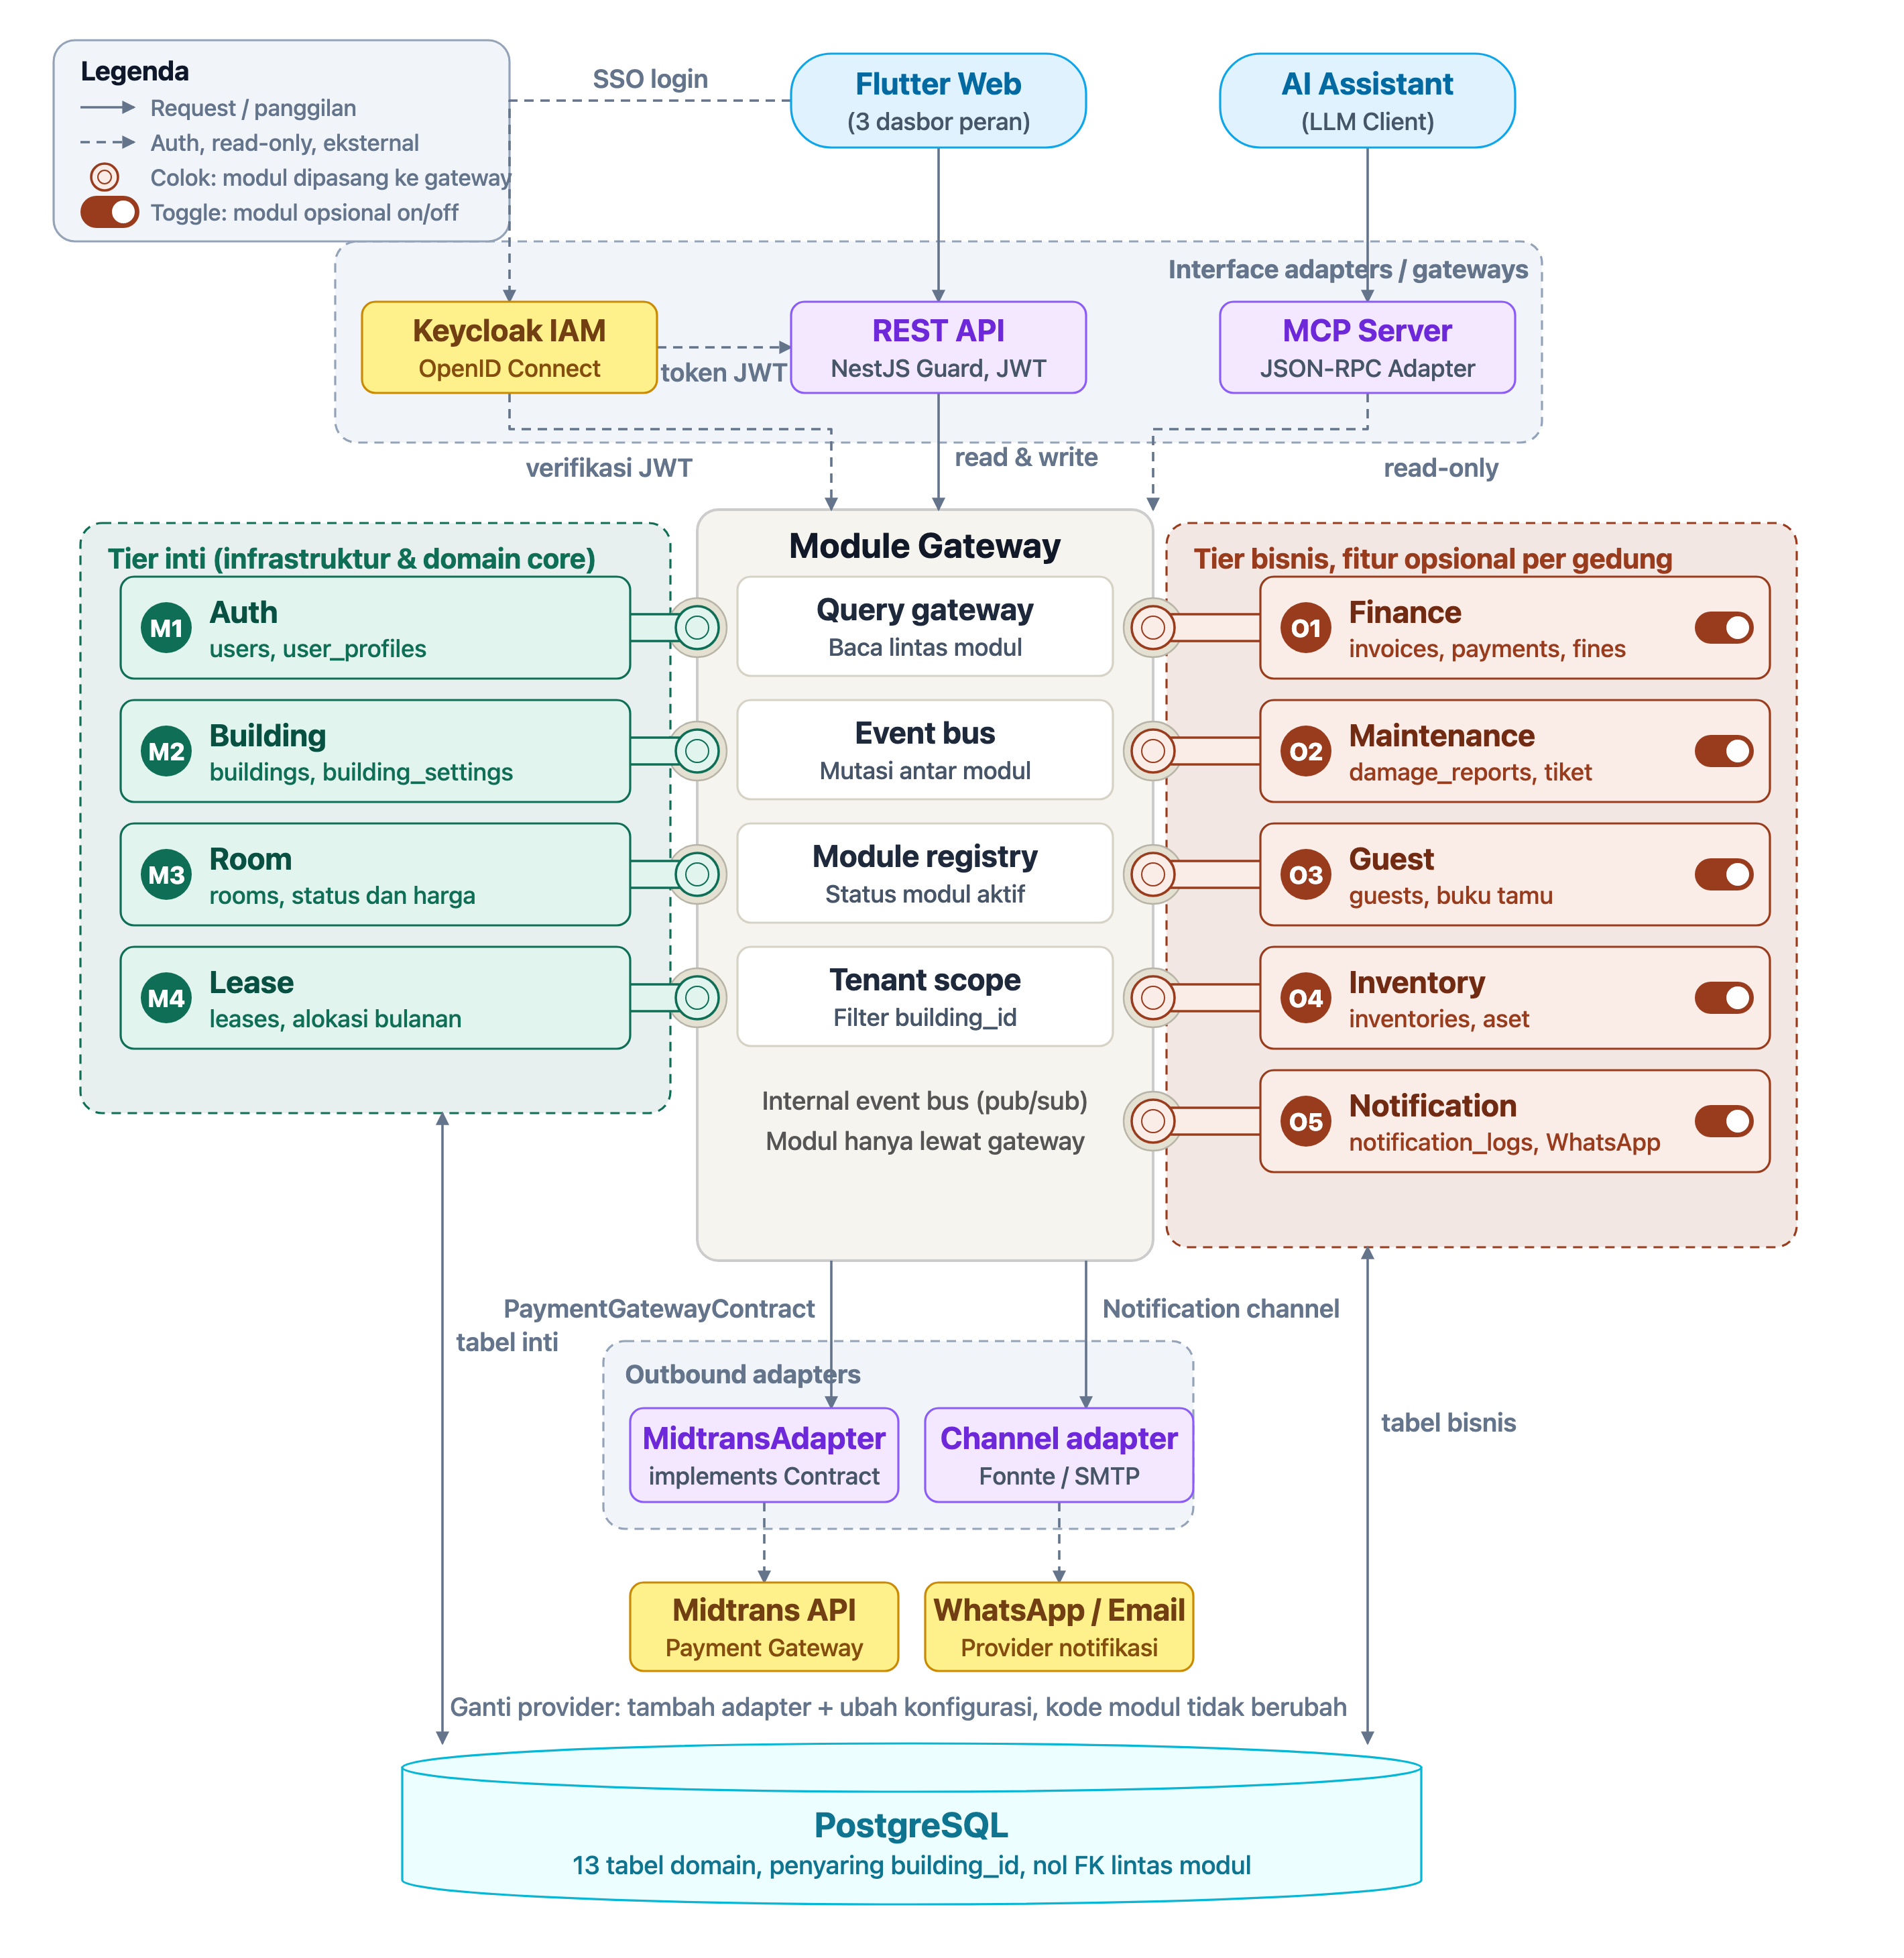
\includegraphics[width=0.9\textwidth,height=0.72\textheight,keepaspectratio]{assets/diagrams/bab2_03_arsitektur_modulith.png}
  \caption{Arsitektur Modular Monolithic}
  \label{fig:teori_modulith}
\end{figure}

\subsection{NestJS}

NestJS adalah kerangka kerja backend berbasis Node.js dan TypeScript yang dirancang untuk membangun aplikasi server dengan struktur modular~\cite{arroziqi2026}. Berbeda dari framework konvensional yang mengharuskan pengembang membuat struktur folder sendiri, NestJS menyediakan pemisahan antar modul sebagai bagian dari kerangka kerjanya. Setiap unit kerja dibungkus dekorator \texttt{@Module()} yang menentukan layanan mana yang boleh diekspor ke modul lain dan mana yang disembunyikan di dalam modul tersebut.

Dua mekanisme membuat hal itu bekerja, sebagaimana diilustrasikan pada Gambar~\ref{fig:teori_nestjs}. Pertama, \textit{encapsulation}: layanan yang tidak didaftarkan pada daftar \texttt{exports} tidak akan pernah bisa disuntik oleh modul lain meskipun keduanya berada di repositori yang sama. Kedua, \textit{dependency injection}: setiap kelas menerima dependensinya dari wadah aplikasi, bukan membuatnya sendiri, sehingga mudah diganti dengan tiruan saat pengujian. Selain itu, NestJS dibangun di atas Node.js yang bekerja dengan model I/O \textit{non-blocking}, sehingga permintaan yang menunggu jawaban dari layanan luar tidak menahan proses lain.

Proyek Akhir ini memilih NestJS karena pemisahan antar modul ditegakkan oleh kerangka kerjanya sendiri, bukan oleh disiplin tim. Ketika modul keuangan mencoba menulis kueri ke tabel milik modul kamar, kode itu akan gagal sejak tahap \textit{build}, bukan baru ketahuan saat pengujian. Pengalaman sistem lama menunjukkan bahwa pemisahan yang hanya dijaga lewat aturan tertulis akan cepat dilanggar ketika waktu pengembangan sedang menekan. Dengan NestJS, pelanggaran aturan menjadi kesalahan teknis, bukan pilihan penyusun kode.

\begin{figure}[H]
  \centering
  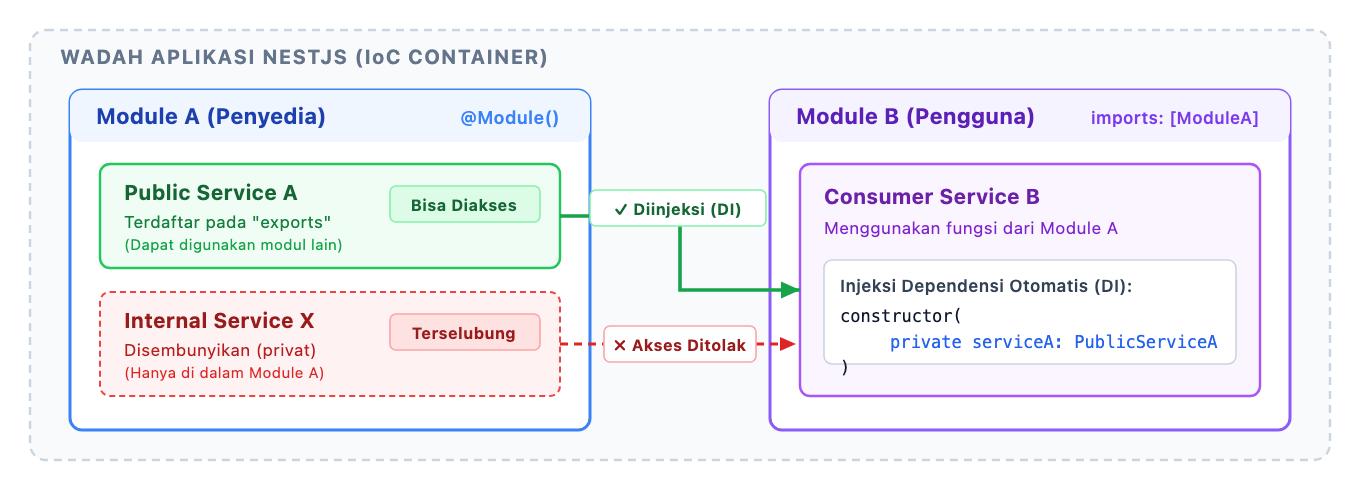
\includegraphics[width=0.92\textwidth,height=0.65\textheight,keepaspectratio]{assets/diagrams/bab2_04_nestjs_modul_di.png}
  \caption{Struktur Modul dan Dependency Injection pada NestJS}
  \label{fig:teori_nestjs}
\end{figure}

\subsection{Flutter}

Flutter adalah kerangka kerja antarmuka lintas platform yang dikembangkan oleh Google dengan bahasa pemrograman Dart~\cite{flutter2025}. Semua tampilan pada aplikasi disusun dari komponen bernama \textit{widget}. Satu basis kode yang sama dapat dikompilasi menjadi aplikasi web, aplikasi Android, maupun aplikasi iOS tanpa menulis ulang lapisan tampilannya. Karena itu Flutter disebut multi-platform, sebab satu proyek dapat dipakai untuk beberapa perangkat sekaligus.

Proyek Akhir ini memakai Flutter dengan target utama berupa aplikasi web. Alasan memilih lingkungan web adalah lingkup penggunaan sistem: pengoperasian harian dilakukan dari komputer atau tablet di ruang pengelola, sehingga tampilan lebar lebih sesuai. Arsitektur yang dipakai juga memperjelas alasan itu. Karena logika bisnis disimpan di lapisan domain yang murni Dart tanpa bergantung pada sistem operasi maupun peramban, lapisan tersebut tetap bisa dipakai ulang ketika aplikasi dikompilasi untuk perangkat mobile di kemudian hari. Jadi kesiapan ekspansi ke mobile muncul sebagai hasil dari struktur kode, bukan sebagai target tambahan yang harus dirancang terpisah.

\subsection{Clean Architecture}

Clean Architecture adalah pola arsitektur yang memisahkan program menjadi lapisan-lapisan dengan aturan ketergantungan satu arah~\cite{martin2017}. Lapisan paling dalam berisi entitas dan aturan bisnis yang murni, lapisan tengah berisi \textit{use case}, dan lapisan luar menangani presentasi serta akses data. Aturan utamanya sederhana: lapisan dalam tidak boleh mengenal keberadaan lapisan luar.

Pada aplikasi Flutter, pemisahan ini menjawab satu masalah yang sering muncul. Kode pada lapisan tampilan biasanya mengambil data langsung dari \textit{repository}, sehingga logika bisnis ikut bercampur dengan komponen antarmuka. Akibatnya, menguji sebuah aturan bisnis berarti menyalakan seluruh tampilan beserta koneksi jaringan. Dengan Clean Architecture, aturan bisnis berdiri sendiri tanpa framework apa pun, sehingga bisa diuji dalam hitungan milidetik.

Proyek Akhir ini memakai Clean Architecture pada sisi antarmuka (Gambar~\ref{fig:teori_clean_arch}) karena pemisahan tersebut memudahkan dua hal. Pertama, pengujian: setiap lapisan punya fokus yang jelas, sehingga aturan bisnis dapat diuji tanpa lapisan lain, dan pengujian antarmuka cukup memeriksa pemetaan \textit{state} ke tampilan. Kedua, perubahan pada bagian tertentu tidak menimpa bagian lain. Contohnya, apabila format jawaban API berubah, cukup ubah lapisan data; lapisan domain dan lapisan presentasi tidak perlu disentuh karena keduanya tidak tahu bentuk data mentah.

\begin{figure}[H]
  \centering
  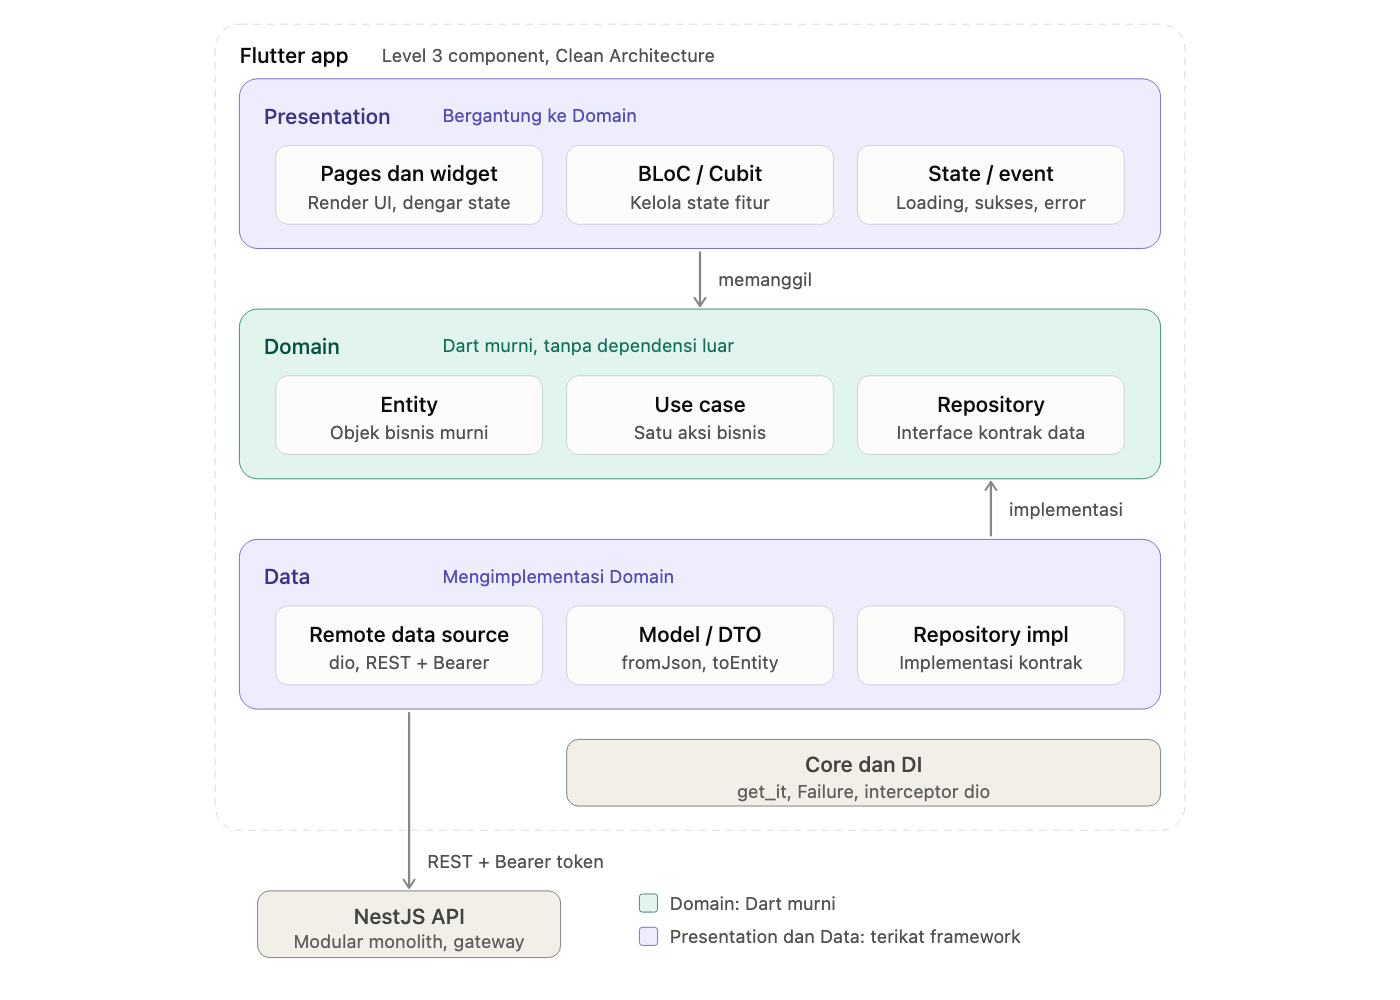
\includegraphics[width=0.82\textwidth,height=0.68\textheight,keepaspectratio]{assets/diagrams/bab2_05_flutter_clean_arch.png}
  \caption{Penerapan Clean Architecture pada Aplikasi Flutter}
  \label{fig:teori_clean_arch}
\end{figure}

\subsection{BLoC (Business Logic Component)}

BLoC adalah pola pengelolaan \textit{state} pada Flutter yang memisahkan pemicu perubahan \textit{state} dari proses perubahannya~\cite{flutter2025}. Alurnya sederhana, seperti terlihat pada Gambar~\ref{fig:teori_bloc}: widget mengirim \textit{event}, \textit{bloc} yang menerima \textit{event} itu memanggil \textit{use case}, lalu \textit{bloc} memancarkan \textit{state} baru dalam bentuk objek yang tidak bisa diubah setelah dibuat.

Pola ini membuat aliran data pada antarmuka berjalan satu arah dan mudah dilacak. Urutannya dapat dibaca langsung dari kode: dari widget, ke \textit{event}, ke \textit{use case}, ke \textit{state}, lalu kembali ke widget. Berbeda dengan pemanggilan \texttt{setState} yang menyatukan pemicu dan perubahan di dalam satu widget, BLoC memisahkannya sehingga transisi \textit{state} bisa diuji tanpa menampilkan antarmuka sama sekali.

Proyek Akhir ini memakai BLoC karena pola ini sebenarnya memaksa struktur kode menjadi tertata. BLoC hanya bekerja jika logika bisnis berada di \textit{use case} terpisah dari widget yang memunculkannya. Umumnya, pengembang yang langsung memuat data dan memprosesnya di dalam widget akan membuat pola ini mustahil diterapkan. Dengan BLoC, pemisahan antara logika bisnis dan tampilan bukan lagi pilihan disiplin, melainkan syarat agar pola tersebut berjalan.

\begin{figure}[H]
  \centering
  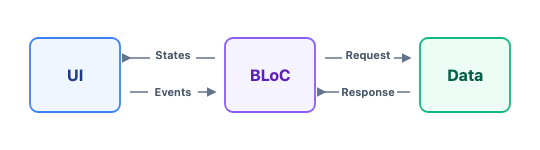
\includegraphics[width=0.72\textwidth,height=0.45\textheight,keepaspectratio]{assets/diagrams/bab2_06_bloc_flow.png}
  \caption{Alur Pengelolaan State Menggunakan Pola BLoC}
  \label{fig:teori_bloc}
\end{figure}

\subsection{PostgreSQL}

PostgreSQL adalah sistem manajemen basis data relasional \textit{open-source} yang dikenal konsisten dengan standar SQL, mendukung transaksi dengan integritas tinggi, dan menyediakan penanganan konkurensi yang matang~\cite{postgresql2023}. Yang membedakannya dari basis data relasional lain terletak pada tiga hal yang dipakai langsung pada sistem ini.

Pertama, tipe numerik \texttt{NUMERIC} dipakai untuk seluruh nilai uang. Tipe ini menyimpan angka desimal secara tepat, sehingga penjumlahan tagihan tidak pernah menghasilkan selisih satu rupiah akibat pembulatan. Kedua, tipe \texttt{JSONB} dipakai untuk menyimpan \textit{payload event} dan parameter \textit{tool} MCP, sekaligus memudahkan pencarian di dalam struktur tersebut. Ketiga, PostgreSQL menyediakan penguncian baris dengan \texttt{SELECT ... FOR UPDATE}, yaitu mengunci baris yang sedang dibaca selama transaksi masih berjalan.

Mekanisme penguncian itulah yang dipakai untuk mencegah dua orang memesan kamar yang sama pada saat bersamaan. Saat permintaan sewa masuk, baris kamar dikunci lebih dulu, lalu diperiksa apakah sudah ada kontrak aktif di periode tersebut. Kalau belum ada, kontrak disimpan di dalam transaksi yang sama; kalau sudah ada, transaksi dibatalkan dan permintaan kedua ditolak. Selama penguncian masih aktif, permintaan lain untuk kamar yang sama harus mengantre. Inilah yang membuat pemesanan ganda tidak mungkin terjadi meski beberapa orang menekan tombol sewa pada milidetik yang sama.

\subsection{Multi-Tenancy dengan Row-Level Scoping}

Dalam pengembangan aplikasi berbasis \textit{SaaS} (\textit{Software as a Service}) untuk properti multi-gedung, pemilihan model \textit{multi-tenancy} menentukan bagaimana data antar-gedung (\textit{tenant}) diisolasi dalam satu ekosistem \textit{backend}. Secara arsitektur, terdapat dua pendekatan utama dalam menangani pemisahan data ini: \textit{Database-Level Isolation} (pemisahan database fisik per gedung) dan \textit{Application-Level Isolation} melalui \textit{Shared Database with Row-Level Scoping}.

Pendekatan pertama memberikan isolasi tingkat tinggi, namun tidak efisien secara operasional karena setiap penambahan gedung baru menuntut migrasi skema terpisah dan membebani pengelolaan koneksi basis data. Oleh karena itu, Proyek Akhir ini menerapkan model \textbf{Shared Database dengan Row-Level Scoping} berbasis kolom penanda \texttt{building\_id}, sebagaimana ditunjukkan pada Gambar~\ref{fig:teori_multitenant}.

\begin{enumerate}[label=\arabic*., leftmargin=*]
  \item \textbf{Efisiensi Migrasi Skema:} Perubahan struktur tabel atau pembaruan migrasi basis data cukup dieksekusi sekali secara global tanpa perlu mengulang skrip migrasi per database gedung.
  \item \textbf{Optimalisasi Agregasi Portofolio:} Pemilik properti membutuhkan laporan keuangan dan tingkat okupansi lintas gedung secara \textit{real-time}. Dengan basis data bersama, laporan gabungan dapat ditarik menggunakan kueri agregasi tunggal tanpa mekanisme \textit{distributed join}.
  \item \textbf{Integritas di Lapisan Aplikasi:} Isolasi data ditegakkan secara ketat melalui penambahan filter \texttt{building\_id} secara otomatis pada setiap kueri ORM di tingkat \textit{backend} NestJS, yang dipetakan langsung dari klaim token akses JWT pengguna.
\end{enumerate}

\begin{figure}[H]
  \centering
  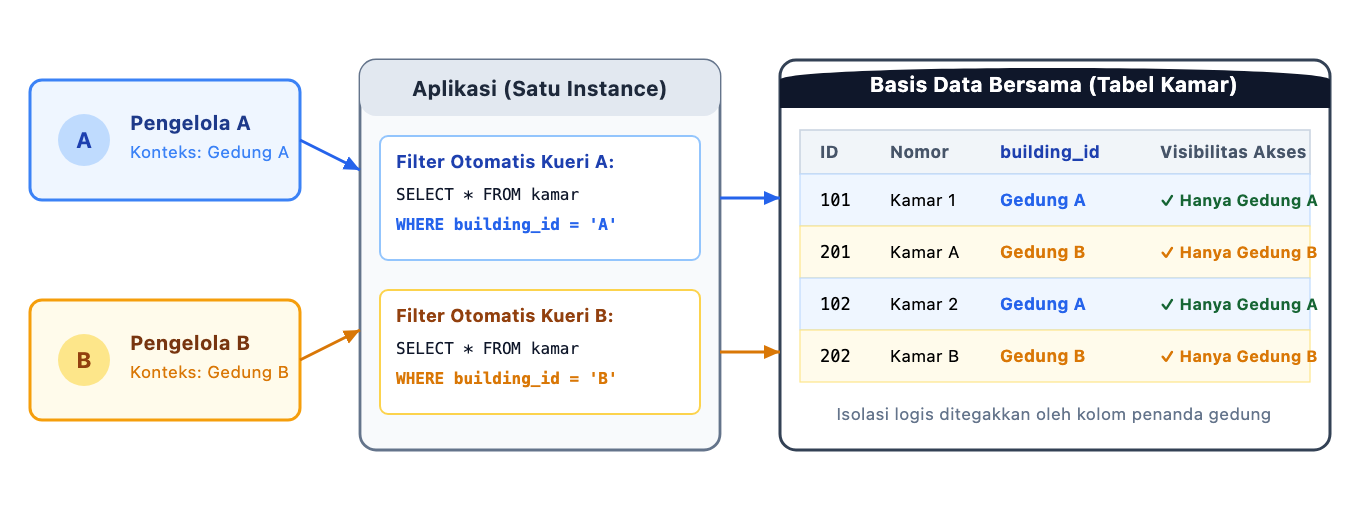
\includegraphics[width=0.92\textwidth,height=0.55\textheight,keepaspectratio]{assets/diagrams/bab2_07_row_level_scoping.png}
  \caption{Pendekatan Multi-Tenancy Shared Database dengan Row-Level Scoping}
  \label{fig:teori_multitenant}
\end{figure}

\subsection{Single Sign-On, OpenID Connect, dan Keycloak}

Single Sign-On (SSO) adalah mekanisme yang memungkinkan pengguna cukup sekali masuk untuk mengakses beberapa aplikasi sekaligus tanpa mengulang kredensial di setiap aplikasi~\cite{sakimura2014}. Pada sistem yang punya banyak modul atau banyak aplikasi terpisah, mekanisme ini menghemat waktu pengguna sekaligus mengurangi jumlah kata sandi yang harus dikelola.

OpenID Connect (OIDC) adalah standar yang mengatur lapisan identitas di atas OAuth 2.0. Bedanya, OAuth 2.0 hanya mengatur pendelegasian hak akses, sedangkan OIDC menambahkan identitas: setelah pengguna berhasil masuk, aplikasi menerima \textit{token} berisi informasi siapa penggunanya. Token tersebut berbentuk JWT dan ditandatangani secara digital, sehingga pihak lain bisa memastikan token itu benar berasal dari penyedia identitas dan belum kedaluwarsa. Karena tanda tangannya dapat diperiksa tanpa menghubungi server pengeluar token, proses verifikasi bisa dijalankan secara lokal dan cepat.

Keycloak adalah \textit{identity and access management} \textit{open-source} yang mendukung OIDC, SSO, dan pengelolaan peran~\cite{keycloak2025}. Yang sering tidak dikerjakan sendiri oleh aplikasi adalah justru hal-hal standar ini: verifikasi email saat pendaftaran, pemulihan kata sandi ketika pengguna lupa, masa berlaku sesi, dan pencatatan aktivitas login. Pada sistem lama seluruh itu harus dibuat satu per satu, dan bagian yang paling sering tertinggal justru yang paling penting, yaitu pemulihan akun.

Proyek Akhir ini memakai Keycloak (Gambar~\ref{fig:teori_oidc}) karena tiga alasan. Pertama, fitur keamanan yang dibutuhkan sudah tersedia sehingga waktu pengembangan bisa dipakai untuk aturan bisnis sewa. Kedua, peran pengguna seperti pemilik, pengelola, dan penghuni cukup diatur di satu tempat, lalu diteruskan ke backend lewat isi token. Ketiga, backend cukup memverifikasi tanda tangan token tanpa perlu menghubungi Keycloak pada setiap permintaan, sehingga waktu tanggap tidak bertambah. Perlu dicatat bahwa Keycloak menambah satu layanan yang harus dijalankan dan dipelihara, dan pembagian peran harus disusun di Keycloak dengan cermat supaya tetap sinkron dengan aturan pada sistem.

\begin{figure}[H]
  \centering
  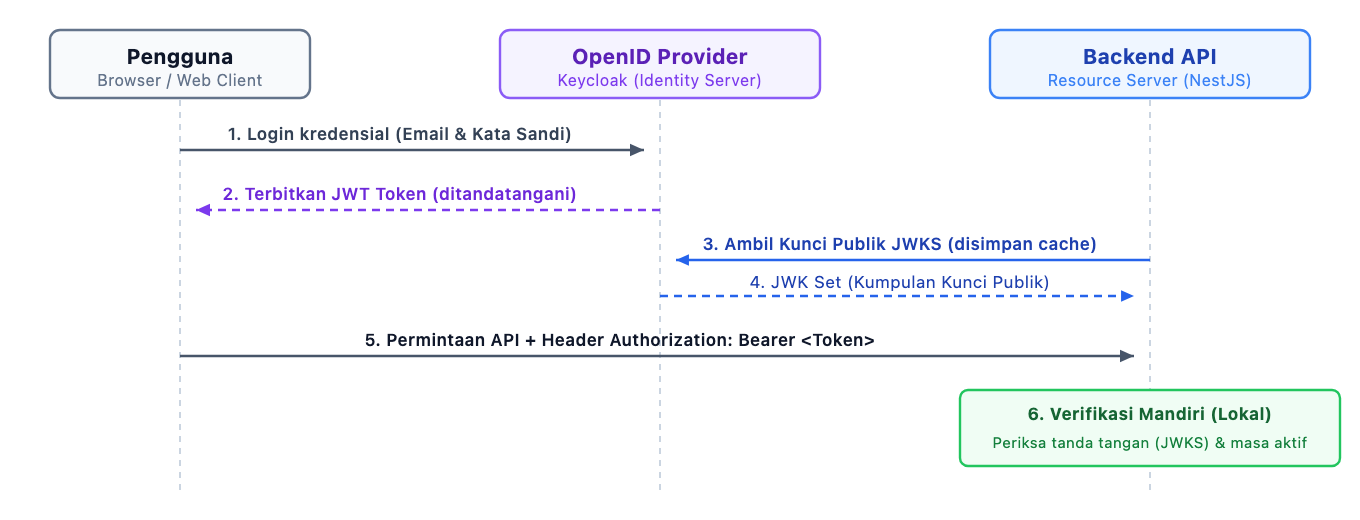
\includegraphics[width=0.92\textwidth,height=0.55\textheight,keepaspectratio]{assets/diagrams/bab2_08_oidc_jwks.png}
  \caption{Alur Autentikasi SSO Berbasis OpenID Connect dengan Keycloak}
  \label{fig:teori_oidc}
\end{figure}

\subsection{Docker dan Docker Compose}

Docker adalah platform \textit{containerization} yang membungkus aplikasi beserta seluruh dependensinya ke dalam satu unit bernama \textit{image}~\cite{merkel2014}. \textit{Image} ini berisi semua yang diperlukan untuk menjalankan aplikasi: kode, pustaka, konfigurasi, sampai sistem operasi dasar. Karena isinya lengkap dan tidak bergantung pada isi mesin, aplikasi yang berjalan di laptop pengembang akan berjalan sama persis di server.

Perbedaan utama Docker dengan cara lama adalah pemisahan antara apa yang ada di kode dan apa yang ada di komputer. Pada pendekatan lama, setiap orang memasang PostgreSQL dan Keycloak dengan versi masing-masing, dan versi yang berbeda sering menyebabkan program berjalan di satu komputer tetapi gagal di komputer lain. Dengan Docker, versi PostgreSQL dan Keycloak dituliskan di satu berkas konfigurasi, lalu dijalankan apa adanya di mana saja.

Docker Compose adalah kelanjutannya. Compose membaca satu berkas yang menjelaskan beberapa container sekaligus, lalu menjalankan semuanya dengan satu perintah. Proyek Akhir ini punya tiga komponen yang harus jalan bersamaan: backend NestJS, basis data PostgreSQL, dan Keycloak. Compose dipakai agar ketiganya bisa dijalankan, dihentikan, dan di-\textit{build} ulang tanpa langkah manual yang berbeda-beda.

\subsection{Midtrans SNAP}

Midtrans adalah penyedia layanan gerbang pembayaran yang menghubungkan aplikasi dengan jaringan pembayaran bank dan dompet digital. Midtrans SNAP merupakan layanan andalannya: SNAP menyediakan antarmuka pembayaran siap pakai dalam bentuk \textit{pop-up}, sehingga penghuni tidak perlu meninggalkan aplikasi untuk menyelesaikan transaksi~\cite{midtrans2025}. SNAP mendukung kanal Virtual Account, QRIS, dan dompet digital.

Integrasi berjalan dua arah, sebagaimana diperlihatkan pada Gambar~\ref{fig:teori_midtrans}. Dari sisi sistem, backend meminta token pembayaran lalu meneruskannya ke antarmuka SNAP, dan penghuni menyelesaikan pembayaran di sana. Dari sisi Midtrans, setiap kali status pembayaran berubah, Midtrans mengirim \textit{webhook} ke alamat yang didaftarkan. Di sinilah bagian yang perlu diperhatikan berada: \textit{webhook} adalah permintaan yang masuk dari luar, sehingga harus diperiksa sebelum dipercayai.

Ada dua perlindungan yang dipakai pada sistem ini. Yang pertama, penomoran pesanan: setiap permintaan pembayaran diberi nomor unik, sehingga ketika gangguan jaringan memicu pengiriman ulang permintaan, Midtrans mengenali bahwa itu transaksi yang sama dan tidak membuat tagihan ganda. Yang kedua, verifikasi tanda tangan: setiap \textit{webhook} disertai tanda tangan yang dihitung dari nomor pesanan, kode status, jumlah pembayaran, dan kunci rahasia. Backend menghitung ulang tanda tangan itu; kalau tidak cocok, permintaan ditolak dan status tagihan tidak diubah. Tanpa dua perlindungan ini, siapa pun yang mengetahui alamat \textit{webhook} bisa memalsukan pembayaran.

\begin{figure}[H]
  \centering
  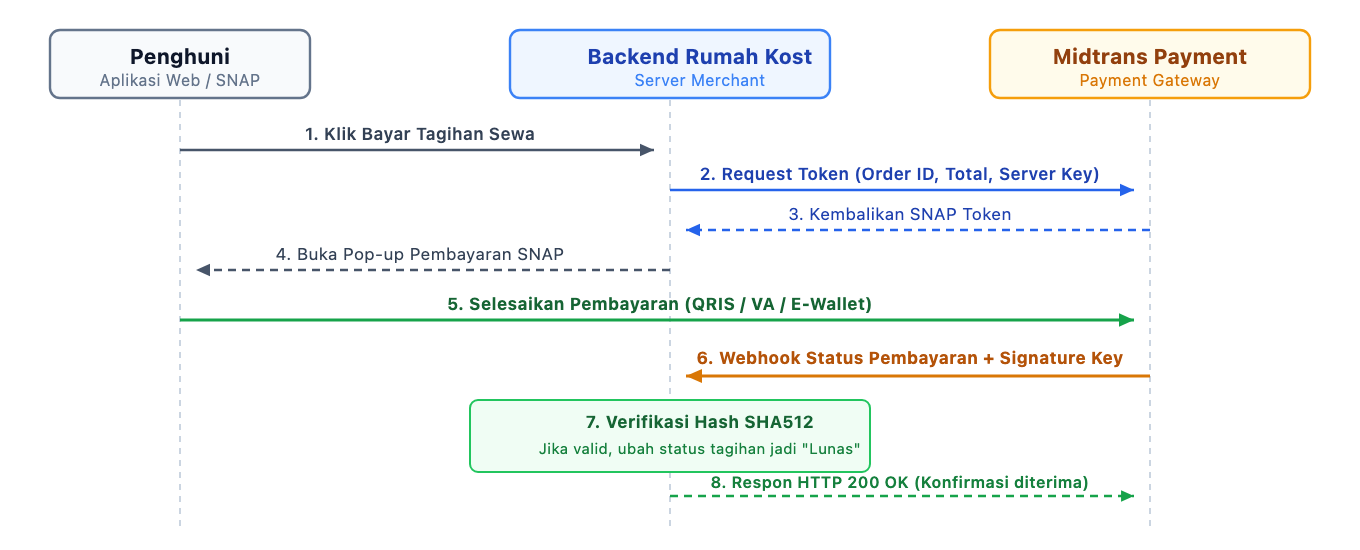
\includegraphics[width=0.92\textwidth,height=0.55\textheight,keepaspectratio]{assets/diagrams/bab2_09_midtrans_webhook.png}
  \caption{Alur Transaksi dan Pembayaran Digital via Midtrans SNAP}
  \label{fig:teori_midtrans}
\end{figure}

\subsection{Standar Kontrak Input-Output REST API}

REST API adalah gaya komunikasi yang paling umum dipakai antaraplikasi web. Yang dikirim berupa permintaan HTTP, dan jawabannya berupa \textit{response} dengan kode status yang menyatakan berhasil atau gagal. Kelemahannya, pengembang kerap membuat format respons secara bebas, sehingga struktur antar-\textit{endpoint} menjadi tidak konsisten. Hal ini membebani lapisan antarmuka (\textit{frontend}) karena harus menangani berbagai pola respons dan pesan galat yang bervariasi secara redundan.

Untuk mengatasi permasalahan tersebut, sistem ini menerapkan standar kontrak input-output yang tersentralisasi melalui \textit{uniform response envelope}. Setiap \textit{endpoint} diatur agar selalu mengembalikan respons dengan lima kunci utama yang seragam: \texttt{status} (menunjukkan status berhasil/gagal), \texttt{message} (keterangan yang dapat dibaca manusia), \texttt{data} (isi \textit{payload} utama), \texttt{meta} (informasi tambahan seperti penomoran halaman), dan \texttt{errors} (rincian kesalahan validasi yang mengacu pada standar \textit{Problem Details}).

Sebagai perbandingan langsung, berikut adalah kontras antara format respons sistem lama yang tidak terstandarisasi dengan format baru yang diterapkan pada kasus pembuatan kontrak sewa (\textit{Create Lease}):

\begin{enumerate}[label=\arabic*., leftmargin=*]
  \item \textbf{Contoh Respons Gagal (\textit{Error} / Gagal Validasi):}
    \begin{enumerate}[label=\alph*., leftmargin=*]
      \item \textit{Format Lama (Tidak Standar):} Setiap \textit{endpoint} mengembalikan struktur yang berbeda-beda dan tidak spesifik pada kolom input yang bermasalah.
\begin{lstlisting}
{
  "success": false,
  "error_message": "Durasi kurang dari minimal gedung dan kamar sudah terisi."
}
\end{lstlisting}
      \item \textit{Format Baru (Sistem Ini --- Standar Problem Details):} Mengembalikan rincian \textit{field} yang mengalami kesalahan validasi (kode HTTP 422) sehingga aplikasi Flutter dapat langsung memetakannya ke masing-masing kolom form input secara presisi.
\begin{lstlisting}
{
  "status": false,
  "message": "Validasi masukan gagal",
  "errors": {
    "duration_months": [
      "Durasi sewa minimal untuk gedung ini adalah 3 bulan."
    ],
    "room_id": [
      "Kamar sedang disewa atau tidak tersedia pada periode tersebut."
    ]
  }
}
\end{lstlisting}
    \end{enumerate}
  \item \textbf{Contoh Respons Berhasil (\textit{Success}):}
    \begin{enumerate}[label=\alph*., leftmargin=*]
      \item \textit{Format Lama (Tidak Standar):} Properti data yang dikembalikan tidak konsisten (kadang menggunakan \texttt{camelCase} atau \texttt{snake\_case} secara acak) dan sering kali hanya mengembalikan ID tanpa rincian objek.
\begin{lstlisting}
{
  "code": 200,
  "msg": "OK",
  "data": 12
}
\end{lstlisting}
      \item \textit{Format Baru (Sistem Ini):} Mengembalikan struktur objek data secara lengkap, konsisten, dan menggunakan kode HTTP 201 (\textit{Created}) untuk data baru.
\begin{lstlisting}
{
  "status": true,
  "message": "Kontrak sewa berhasil dibuat",
  "data": {
    "lease_id": 12,
    "room_number": "A-02",
    "duration_months": 3,
    "total_amount": 2550000,
    "status": "pending"
  }
}
\end{lstlisting}
    \end{enumerate}
\end{enumerate}

Kode status yang dipakai pada sistem ini mengikuti ketetapan umum HTTP:
\begin{enumerate}[label=\arabic*., leftmargin=*]
  \item \textbf{Kode 200 dan 201:} Permintaan berhasil diproses atau data baru berhasil dibuat.
  \item \textbf{Kode 400:} Permintaan tidak sesuai format (\textit{bad request}).
  \item \textbf{Kode 401:} Token autentikasi tidak tersedia atau sudah kedaluwarsa (\textit{unauthorized}).
  \item \textbf{Kode 403:} Pengguna tidak memiliki hak akses (\textit{forbidden}) terhadap data gedung tersebut.
  \item \textbf{Kode 404:} Data yang diminta tidak ditemukan (\textit{not found}).
  \item \textbf{Kode 422:} Masukan data melanggar aturan bisnis (\textit{unprocessable entity}), misalnya durasi sewa di bawah batas minimum gedung.
\end{enumerate}

Dengan seluruh kemungkinan respons yang mengikuti pola amplop seragam ini, sisi antarmuka (\textit{frontend} Flutter Web) cukup menuliskan satu fungsi penanganan global untuk mengelola seluruh status dan galat API secara bersih.

\subsection{Model Context Protocol}

Model Context Protocol (MCP) adalah standar terbuka yang menghubungkan model kecerdasan buatan dengan sumber data dan fungsi di luar model tersebut~\cite{anthropic2024}. Sebagian besar pertanyaan operasional membutuhkan data nyata yang tidak ada di dalam model, sehingga tanpa akses ke data itu model hanya bisa menebak.

MCP menjawab dengan memisahkan tiga peran. \textit{Host} adalah aplikasi yang berinteraksi dengan pengguna, misalnya kolom tanya-jawab pada dasbor. \textit{Client} adalah konektor di dalam host yang meneruskan permintaan ke server. \textit{Server} adalah layanan yang menyediakan data dan fungsi. Ketiganya berkomunikasi memakai pesan JSON-RPC 2.0, yaitu format pertukaran pesan yang sudah disepakati dan tersedia di banyak bahasa pemrograman.

Server MCP mengekspos tiga jenis kemampuan. \textit{Resources} berisi data yang bisa dibaca, misalnya data gedung. \textit{Prompts} berisi templat instruksi, misalnya cara menulis jawaban sebagai analis properti. \textit{Tools} berisi fungsi yang dijalankan model ketika dibutuhkan, misalnya menghitung tingkat keterisian kamar. Karena sebuah \textit{tool} adalah kode yang benar-benar dijalankan, komponen ini harus diperlakukan dengan hati-hati.

Oleh karena itu, pada sistem ini semua \textit{tools} yang diekspos hanya berfungsi membaca, sebagaimana ditunjukkan pada Gambar~\ref{fig:teori_mcp}. Tidak ada satu pun fungsi yang mengubah data. Dengan begitu, jawaban yang muncul di kolom tanya-jawab pasti berdasarkan angka yang benar-benar ada di basis data, dan keputusan penting tetap diambil manusia.

\begin{figure}[H]
  \centering
  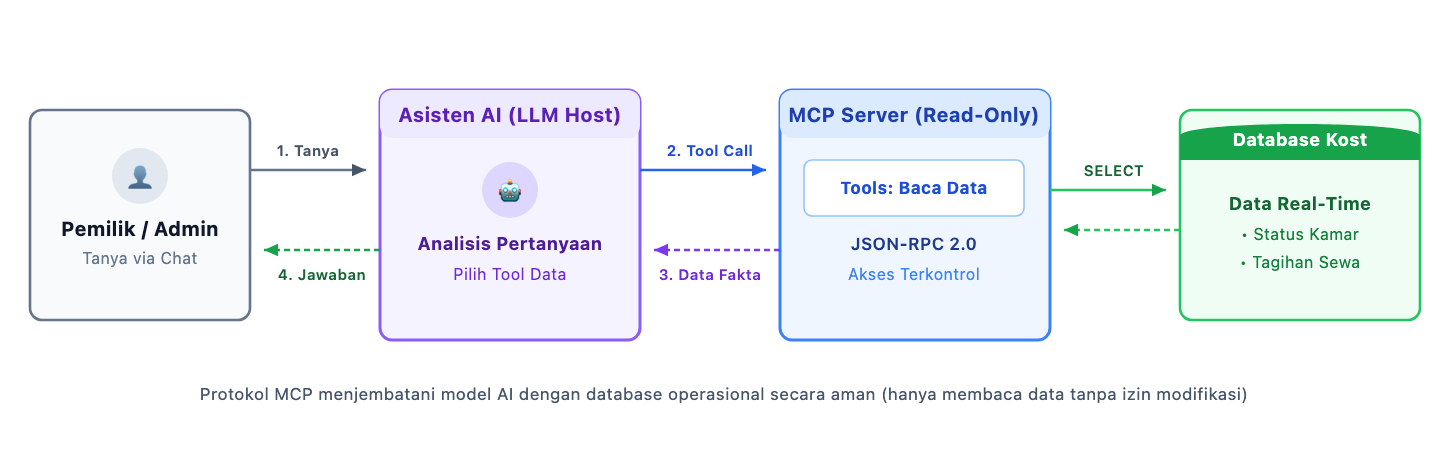
\includegraphics[width=0.92\textwidth,height=0.55\textheight,keepaspectratio]{assets/diagrams/bab2_10_mcp.png}
  \caption{Integrasi Model Context Protocol (MCP) dengan Basis Data Operasional}
  \label{fig:teori_mcp}
\end{figure}

\section{PENELITIAN TERKAIT}
\label{sec:penelitian_terkait}

Beberapa penelitian terdahulu membahas sistem informasi manajemen rumah kost. Penelitian tersebut ditinjau untuk melihat apa yang sudah dikerjakan, apa yang masih menjadi masalah, serta posisi penelitian ini di antaranya.

Penelitian pertama dilakukan oleh Wahyuni pada tahun 2025 dengan judul ``Pengembangan Sistem Informasi Pengelolaan Kos Berbasis Website Dengan Menggunakan Framework Codeigniter''~\cite{wahyuni2025}. Penelitian ini membangun aplikasi web pencatatan data kost. Metode yang digunakan adalah \textit{prototyping} dengan CodeIgniter dan MySQL. Hasilnya berupa aplikasi pencatatan kamar dan penghuni, tetapi hanya mampu mengelola satu gedung dan belum memisahkan hak akses per peran.

Penelitian kedua diterbitkan pada tahun 2025 dengan judul ``Pengembangan Sistem Manajemen Kos Berbasis Aplikasi Mobile pada Kos SidoRame12''~\cite{jati2025}. Metode yang digunakan adalah \textit{prototyping} dengan Flutter dan Laravel. Hasilnya berupa aplikasi mobile dengan pencatatan status kamar dan pengingat pembayaran, tetapi belum mendukung beberapa gedung dan belum ada pengujian otomatis.

Penelitian ketiga dilakukan oleh Ayyubi pada tahun 2024 dengan judul ``Rancang Bangun Sistem Informasi Pembayaran Kost Berbasis Mobile pada Kost WS Barokah Selokaton''~\cite{ayyubi2024}. Penelitian ini membangun layanan pembayaran sewa secara daring. Metode yang digunakan adalah \textit{waterfall} dengan Flutter dan Midtrans SNAP. Hasilnya berupa pembayaran digital, tetapi integrasi Midtrans masih berjalan di lingkungan uji coba tanpa perlindungan terhadap transaksi ganda.

Penelitian keempat diterbitkan pada tahun 2025 dengan judul ``Kelola Kosku''~\cite{jscr2025}. Penelitian ini membangun sistem akuntansi sewa lengkap. Metode yang digunakan adalah MVVM dengan Flutter dan Supabase. Hasilnya mencakup tagihan bulanan otomatis, denda keterlambatan, dan uang jaminan, tetapi memakai basis data non-relasional sehingga integritas transaksi lemah.

Penelitian kelima dilakukan oleh Bintang, Purnamasari, dan Maulana pada tahun 2026 dengan judul ``Transformasi Digital Pengelolaan Kos''~\cite{bintang2026}. Penelitian ini bertujuan mengubah operasional kost menjadi berbasis digital. Metode yang digunakan adalah Scrum dengan Laravel dan Midtrans. Hasilnya berupa penagihan otomatis dan notifikasi WhatsApp, tetapi struktur modul pada backend masih belum tegas.

Penelitian keenam dilakukan oleh Nurfaqih, Budihartono, dan Syefudin pada tahun 2026 dengan judul ``Rancang Bangun Sistem Informasi Manajemen Kost Berbasis Web Menggunakan Framework Laravel''~\cite{nurfaqih2026}. Metode yang digunakan adalah \textit{waterfall} dengan Laravel 12 dan MySQL. Hasilnya berupa aplikasi web dengan ketersediaan kamar langsung, pengingat tagihan, dan tiket komplain, tetapi hanya untuk satu gedung.

Empat proposal \textit{previous work} juga ditinjau sebagai pembanding~\cite{rasyidatur2025,roihanah2025,rizal2025,bagus2025}. Keempatnya memakai Scrum dengan pembagian modul sesuai domain, tetapi pemisahan antar modul tidak ditegakkan.

Berdasarkan telaah tersebut, terlihat pola yang berulang. Sebagian besar sistem hanya mampu melayani satu gedung. Sebagian sudah mengotomasi tagihan tetapi belum menguji tiap modul secara terpisah. Autentikasi masih berupa email dan kata sandi tanpa pemulihan akun. Perbandingan penelitian terkait dirangkum pada Tabel~\ref{tab:penelitian_terkait}.

\begin{longtblr}[
  caption = {Penelitian Terkait},
  label = {tab:penelitian_terkait}
]{
  width = \textwidth,
  colspec = {Q[c,0.7cm] X[1.1,l] X[1.8,l] X[1.2,l] X[2.2,l]}
}
  No & Peneliti \& Tahun & Judul Penelitian & Metode \& Teknologi & Hasil \& Keterbatasan (Gap) \\
  1 & Wahyuni (2025)~\cite{wahyuni2025} & Pengembangan Sistem Informasi Pengelolaan Kos Berbasis Website Dengan Menggunakan Framework Codeigniter Pada Wisma Mutiara Selaras & Prototyping, CodeIgniter, MySQL & Mencatat data kamar dan penghuni berbasis web, tetapi hanya mendukung satu gedung dan belum memisahkan hak akses per peran. \\
  2 & JATI (2025)~\cite{jati2025} & Pengembangan Sistem Manajemen Kos Berbasis Aplikasi Mobile pada Kos SidoRame12 & Prototyping, Flutter, Laravel & Menyediakan pencatatan status kamar dan pengingat pembayaran mobile, tetapi belum mendukung multi-gedung dan tanpa pengujian otomatis. \\
  3 & Ayyubi (2024)~\cite{ayyubi2024} & Rancang Bangun Sistem Informasi Pembayaran Kost Berbasis Mobile pada Kost WS Barokah Selokaton & Waterfall, Flutter, Midtrans SNAP & Menyediakan pembayaran sewa digital, tetapi integrasi Midtrans masih sebatas lingkungan uji coba (\textit{sandbox}) tanpa \textit{idempotency key} dan validasi \textit{webhook}. \\
  4 & JSCR (2025)~\cite{jscr2025} & Kelola Kosku: Sistem Informasi Akuntansi Mobile dengan Anniversary Billing, Auto-Penalty, Security Deposit, dan Depresiasi PMK 72/2023 & MVVM, Flutter, Supabase & Mencakup tagihan bulanan otomatis, denda, dan deposit, namun model bisnis terlalu bercabang dan integritas transaksi relasional lemah. \\
  5 & Bintang dkk. (2026)~\cite{bintang2026} & Transformasi Digital Pengelolaan Kos: Sistem Berbasis Laravel dengan Integrasi Pembayaran Non-tunai & Scrum, Laravel, Midtrans, WhatsApp & Mengotomasi penagihan dan notifikasi WhatsApp, tetapi batas modul pada backend belum ditegakkan secara teknis. \\
  6 & Nurfaqih dkk. (2026)~\cite{nurfaqih2026} & Rancang Bangun Sistem Informasi Manajemen Kost Berbasis Web Menggunakan Framework Laravel & Waterfall, Laravel 12, MySQL & Menyediakan info ketersediaan kamar, pengingat tagihan, dan tiket komplain, tetapi hanya melayani satu gedung tunggal. \\
  7 & Rasyidatur~\cite{rasyidatur2025}, Roihanah~\cite{roihanah2025}, Rizal~\cite{rizal2025}, Bagus~\cite{bagus2025} (2025) & Empat Proposal Sistem Informasi Manajemen Rumah Kost (Penghuni \& Tamu, Kamar \& Reservasi, Keuangan, Operasional) & Scrum, Laravel 11, Flutter, MySQL (41 Tabel) & Modularitas masih semu (\textit{tight coupling} dan FK lintas modul), skema membengkak hingga 41 tabel, hanya satu gedung, dan autentikasi masih primitif. \\
  8 & Bagus Alfian (2026) -- Penelitian Ini & Arsitektur Modular Monolithic Berbasis Event-Driven untuk Sistem Informasi Manajemen Rumah Kost Terintegrasi & Scrum, Modular Monolith NestJS, Flutter Web (Clean Arch), PostgreSQL, Keycloak OIDC, MCP & 9 modul terenkapsulasi (nol FK lintas modul), multi-gedung (\textit{row-level scoping}), sewa bulanan fleksibel per gedung, SSO Keycloak, Midtrans idempoten, dan asisten AI via MCP \textit{read-only}. \\
\end{longtblr}

\subsection{Sintesis dan Gap Statement}

Berdasarkan telaah atas penelitian terkait pada Subbab~\ref{sec:penelitian_terkait} dan evaluasi terhadap empat proposal \textit{previous work}, ditemukan lima kesenjangan yang belum diselesaikan oleh penelitian terdahulu.

\subsubsection{1. Modular Monolithic yang Belum Diterapkan dengan Benar}

Hampir semua penelitian yang memakai istilah \textit{modular monolithic} pada Tabel~\ref{tab:penelitian_terkait} membaginya hanya pada level struktur folder. Modul keuangan tetap bisa membaca tabel modul kamar secara langsung. Relasi \textit{Foreign Key} juga dipasang melintasi batas domain. Akibatnya, tidak ada bagian yang bisa diuji atau dilepas tanpa menarik bagian lain. Empat \textit{previous work} mengalami hal yang sama~\cite{rasyidatur2025,roihanah2025,rizal2025,bagus2025}.

Masalahnya bukan pada istilah yang dipakai, melainkan pada cara penerapannya. Pemisahan antar modul yang hanya berupa kesepakatan tertulis akan dilanggar ketika waktu pengembangan sedang menekan. Pada penelitian kost, pemisahan yang dipaksakan oleh kerangka kerja belum pernah dipakai.

\subsubsection{2. Hanya Mendukung Satu Gedung}

Tiga dari enam penelitian eksternal pada Tabel~\ref{tab:penelitian_terkait} menghasilkan sistem untuk satu gedung fisik. Ketika pemilik menambah properti, satu-satunya pilihan adalah memasang instalasi dan basis data terpisah untuk setiap gedung~\cite{wahyuni2025,jati2025,nurfaqih2026}. Akibatnya, laporan gabungan seluruh portofolio tidak bisa disusun tanpa menggabungkan data dari beberapa tempat.

\subsubsection{3. Autentikasi Masih Bersifat Primitif}

Semua penelitian pada Tabel~\ref{tab:penelitian_terkait} mengelola kredensial pengguna secara mandiri di dalam basis data. Tidak satu pun menyediakan verifikasi email, pemulihan kata sandi, dan manajemen sesi yang terstandarisasi. Akibatnya, risiko kebocoran akun tinggi, dan waktu pengembangan tersedot untuk membangun fitur keamanan yang seharusnya tersedia siap pakai~\cite{rasyidatur2025,roihanah2025,rizal2025,bagus2025}.

\subsubsection{4. Model Sewa Terlalu Bercabang}

Kelola Kosku, misalnya, menangani tagihan bulanan otomatis, denda keterlambatan, dan uang jaminan sekaligus~\cite{jscr2025}. Fitur itu dibuat sangat lengkap, sementara fitur lain pada sistem yang sama masih sederhana. Justru kedalaman satu fitur inilah yang menjadi masalah. Model bisnis yang bercabang memaksa skema basis data ikut bercabang.

Pada \textit{previous work}, hal ini terlihat paling jelas. Sistem harus melayani satuan sewa harian, bulanan, dan tahunan sekaligus, sampai basis data tumbuh menjadi empat puluh satu tabel dengan banyak kolom yang sudah tidak dipakai~\cite{rasyidatur2025,roihanah2025,rizal2025,bagus2025}. Kesenjangan ini bukan pada jumlah fiturnya, melainkan pada cara aturan bisnisnya ditata. Aturan yang berbeda antar gedung lebih tepat disimpan sebagai konfigurasi.

\subsubsection{5. Belum Tersedia Jawaban Cepat lewat Asisten \textit{Artificial Intelligence}}

Pemilik kost sering butuh jawaban cepat: berapa tingkat keterisian kamar bulan ini, atau siapa yang sedang menunggak. Pada penelitian terdahulu, jawaban itu harus dihimpun dengan membuka beberapa halaman satu per satu. Belum ada penelitian sistem manajemen kost yang menyediakan akses baca lewat protokol standar yang menghubungkan model \textit{Artificial Intelligence} dengan data operasional.

\textit{Model Context Protocol} menyediakan jalan keluar. Protokol ini memungkinkan model \textit{Artificial Intelligence} memanggil fungsi baca pada data operasional. Batasannya jelas: fungsi yang diekspos hanya membaca dan tidak mengubah apa pun. Dengan begitu, jawaban yang muncul selalu berdasarkan angka yang benar-benar ada.

Proyek Akhir ini menjawab kelima kesenjangan tersebut melalui perancangan \textbf{Sistem Informasi Manajemen Rumah Kost Berbasis Arsitektur Modular Monolithic}. Pemisahan antar modul ditegakkan oleh kerangka NestJS sehingga tiap bagian bisa diuji terpisah. Sistem dirancang untuk beberapa gedung, bukan satu gedung. Autentikasi memakai standar industri agar pemulihan kata sandi dan verifikasi email tidak dibangun dari nol. Model bisnis disederhanakan menjadi sewa bulanan dengan aturan per gedung. Jawaban cepat disediakan lewat \textit{Model Context Protocol} dengan model \textit{Artificial Intelligence} yang hanya bisa membaca data.
